\documentclass[12pt]{article}
\usepackage[dvips]{epsfig}
\usepackage{url}
\usepackage[colorlinks=true]{hyperref}

\begin{document}

\section*{GENESIS: Documentation}

{\bf Related:}
% start: userdocs-tag-replace-items related-do-nothing
% end: userdocs-tag-replace-items related-do-nothing

\section*{The GENESIS Publication System}

A powerful feature of the GENESIS software system is the capacity to track the life cycle of a research project, from creation through development and extension to publication.

\subsection*{Introduction}

The following figure illustrates the global workflows and dataflows that support the GENESIS publication system.

\begin{figure}[h]
  \centering
   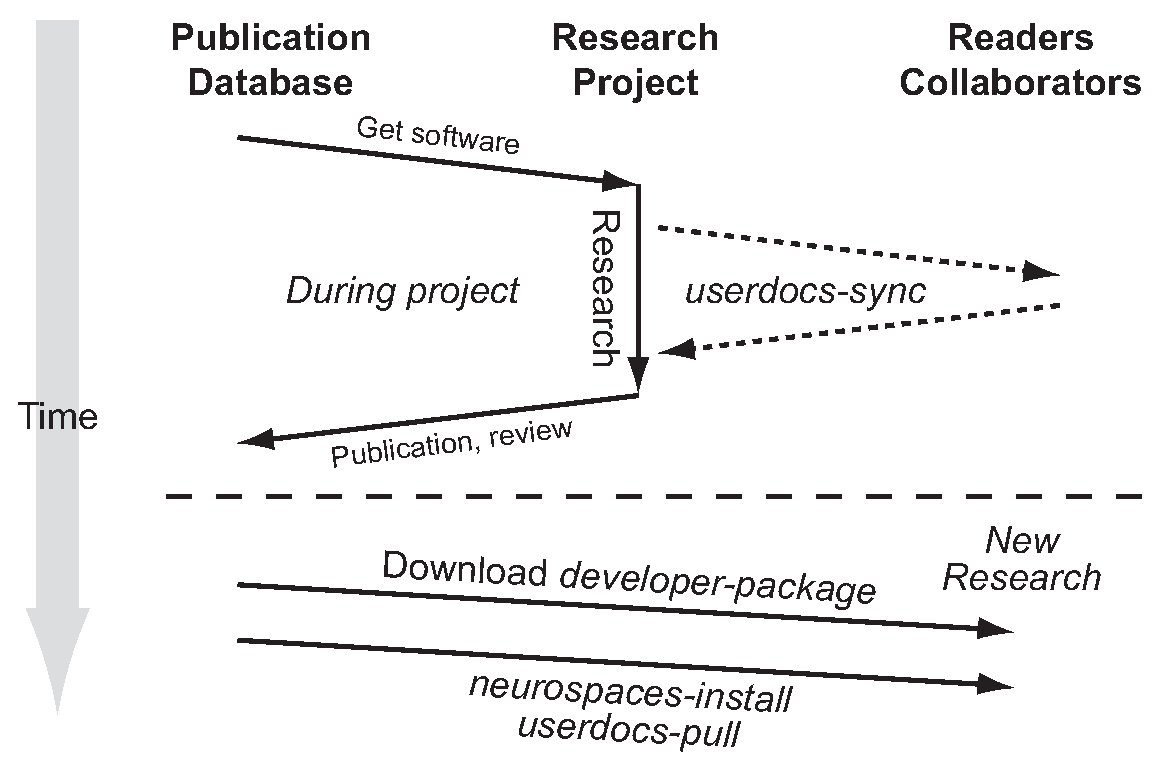
\includegraphics[scale=0.6]{figures/global-workdata-flow.eps}
%\caption{{\bf A Dummy Figure:} Example of \LaTeX\,\,\,code to incorporate a figure into documentation.}
  \label{fig:wf-1}
\end{figure}

% \subsection*{Steps in Document Publication}


UNDER CONSTRUCTION

\end{document}